\chapter{Testing}

\section{Test Plan}

\begin{landscape}
\subsection{Original Outline Plan}

\begin{center}
    \begin{tabular}{|p{2cm}|p{5cm}|p{5cm}|p{4cm}|}
        \hline
        \textbf{Test Series} & \textbf{Purpose of Test Series} & \textbf{Testing Strategy} & \textbf{Strategy Rationale}\\ \hline
        1 & Testing the flow of control between user interfaces & Top-down Testing & \\ \hline
        2 & Testing the validation of input data & Bottom-up testing & All components are to be tested after development \\ \hline
        3 & Testing the algorithms' functionality & White box testing & \\ \hline
        4 & Testing that the information has been successfully stored, and in the right places & Black box testing & \\ \hline
        5 & Testing the system and whether it meets the requirements & System testing & \\ \hline
    \end{tabular}
\end{center}


\subsection{Changes to Outline Plan}

\begin{center}
    \begin{tabular}{|p{2cm}|p{5cm}|p{5cm}|p{4cm}|}
        \hline
        \textbf{Test Series} & \textbf{Purpose of Test Series} & \textbf{Testing Strategy} & \textbf{Strategy Rationale}\\ \hline 
        1 & Testing the flow of control between user interfaces & Top-down Testing & \\ \hline
        2 & Testing the validation of input data & Bottom-up testing & All components are to be tested after development \\ \hline
        3 & Testing the algorithms' functionality & White box testing & \\ \hline
        4 & Testing that the information has been successfully stored, and in the right places & Black box testing & \\ \hline
        5 & Testing the system and whether it meets the requirements & System testing & \\ \hline
    \end{tabular}
\end{center}

\subsection{Original Detailed Plan}


\begin{center}
    \begin{longtable}{|p{1.5cm}|p{2cm}|p{2.5cm}|p{2.5cm}|p{2cm}|p{2cm}|p{2cm}|p{2cm}|}
        \hline
        \textbf{Test Series} & \textbf{Purpose of Test} & \textbf{Test Description} & \textbf{Test Data} & \textbf{Test Data Type (Normal/ Erroneous/ Boundary)} & \textbf{Expected Result} & \textbf{Actual Result} & \textbf{Evidence}\\ \hline
        1.1 & Test the Log in button on the log in screen & This should check whether the password and email match and exist in a record & Click the log in button & Normal & If the email and password match, the main menu should open, else the program should prompt the user with an error & & \\ \hline
        1.2 & Test the View button on the main menu & This button links the main menu to the view menu. & Click the View Button & Normal & The program should open the View Menu in a new window & & \\ \hline
        1.3 & Testing the Log Out button on the Main Menu & This button links to the Login screen, where the user is required to log in again & Click the Log out button & Normal & The screen should switch to the log out screen & & \\ \hline
        1.4 & Testing the Search Database button on the Main Menu & This button should prompt a seperate interface to open, and show details which can be used to search for specific items in the database & Click the Search Database button & Normal & The program should open a new window consisting of the Search Database screen & & \\ \hline
        1.5 & Testing the Add Entry button on the Main Menu & This button should prompt a seperate interface to open and show the Add Entry screen & Click the Add Entry button & Normal & The program should open the Add Entry screen in a new window & & \\ \hline
        1.6 & Testing the Edit Entry button from the Main Menu & This button links to the Editing screen & Click the Edit Entry button & Normal & The program should switch to the Editing screen from the Main Menu &  & \\ \hline
        1.7 & Testing the Edit Entry button after an entry has been selected beforehand & These conditions should open the Edit Entry screen upon clicking Edit Entry, with data on the selected entry already filled in on the grid & Click on an entry, and then click Edit Entry & Normal & The program should open the Edit Entry screen in a new window & & \\ \hline
        1.8 & Testing the Remove Entry Button after an entry has been selected beforehand & These conditions should prompt the user for verification on deleting a selected customer record & Click on an entry and then click Remove Entry & Normal & The program should open a Verification window, asking the user for confirmation and verification on removing the selected customer record & & \\ \hline
        1.9 & Testing the Change Password Button on the Main Menu & This button prompts the Change Password window to open & Click the Change Password button & Normal & The program should open the Change Password window, with fields required to be filled in in order to change the password & & \\ \hline
        1.10 & Testing the Quick Search button on the Main Menu & This button returns the customer that matches the entered AuthorID & Type in a Lastname and click QuickSearch & Normal & The program should return the customer that matches the entered Lastname and show it in the grid & & \\ \hline
        1.11 & Testing the back button on the View Menu & This button returns back to the main menu & Click Back & Normal & The program should return back to the main menu & & \\ \hline
        1.12 & Testing the Add Book Button on the View Menu & This button opens up a new window for adding a book & Click Add Book & Normal & The program should open a new window for adding a book & & \\ \hline
        1.13 & Testing the View Publishing Invoice button on the View Menu & This button opens up a new window displaying details about the selected book's publishing invoice & Click View Publishing invoice & Normal & The program should open a new window containing details about the selected book's publishing invoice & & \\ \hline
        1.14 & Testing the View Royalties button on the View Menu & This button opens up a new window displaying details about the selected book's royalties & Click View Royalties & Normal & The program should open a new window containing details about the selected book's royalties & & \\ \hline
        1.15 & Testing the View Book Invoice button on the View Menu & This button opens up a new window displaying details about the selected book's book invoices & Click View Book Invoices & Normal & The program should open a new window containing details about the selected book's book invoices & & \\ \hline
        1.16 & Testing the Delete book button on the View Menu & This button opens up a new window asking for verification on deleting a selected book record & Click Delete book & Normal & The program should open a Verification window, asking the user for confirmation and verification on removing the selected customer record & & \\ \hline
        2.1 & Verify that some criteria has been entered when using the search & At least one set of the input boxes and dropdown lists must have been filled in or selected from, else the program will prompt the user about the error & Selected from list with names and values entered \newline Selected from list, values enteredand no names entered \newline Just values entered \newline Nothing   & Normal \newline Normal \newline Erroneous \newline Erroneous & Accept \newline Accept \newline Error \newline Error & & \\ \hline
        2.2 & Verify that a valid email has been entered on the log in screen &  The program will prompt the user telling them they have inputted an error & test@testmail.com \newline helloworld \newline test @testmail.com \newline test.com@testmail & Normal \newline Erroneous \newline Erroneous \newline Erroneous & Accept \newline Error \newline Error \newline Error & & \\ \hline
        2.3 & Verify that a valid Firstname has been entered when adding an entry & The user will be prompted with an error & John \newline Jo hn \newline Jo?hn \newline Jo2n & Normal \newline Erroneous \newline Erroneous \newline Erroneous & Accept \newline Error \newline Error \newline Error & & \\ \hline
        2.4 & Verify that a valid Lastname has been entered when adding an entry & The user will be prompted with an error & Smith \newline Sm ith \newline Smi!th \newline Smi1th & Normal \newline Erroneous \newline Erroneous \newline Erroneous & Accept \newline Error \newline Error \newline Error & & \\ \hline
        2.5 & Verify that a valid Phonenumber has been entered when adding an entry & The user will be prompted with an error & 07123456789 \newline 07123123.3 \newline 071CO2 & Normal \newline Erroneous \newline Erroneous & Accept \newline Error \newline Error & & \\ \hline
        2.7 & Verify that a valid Address has been entered when adding an entry & The user will be prompted with an error & 1 Example road \newline @@~£! \newline 1231231 & Normal \newline Erroneous \newline Erroneous & Accept \newline Error \newline Error & & \\ \hline
        2.8 & Verify that a valid ISBN has been entered when adding a book & The user will be prompted with an error & 1234567890123 \newline @@~£! \newline 123 \newline HelloWorld & Normal \newline Erroneous \newline Erroneous \newline Erroneous & Accept \newline Error \newline Error \newline Error & & \\ \hline
        2.9 & Verify that a valid NoOfPages has been entered when adding a book & The user will be prompted with an error & 123 \newline 123456789 \newline 2.3 \newline @! \newline HelloWorld & Normal \newline Erroneous \newline Erroneous \newline Erroneous & Accept \newline Error \newline Error& & \\ \hline
        3.1 & Verify that all fields required are entered when adding a book & If all fields are filled in correctly, a book will be successfully added to the database & Fill all Fields Correctly and then click Add to Database \newline Leave Fields Blank and then click Add to Database & Normal \newline Erroneous & Verification screen should open \newline User will be prompted with an error & & \\ \hline
        3.2 & Verify that all fields required are entered and calculations are complete when adding an Invoice Item & If all fields are filled in correctly and the calculations are complete, then the invoice item will be added to the database & Fill all fields correctly and click calculate and then click Add to Database \newline Leave Fields Blank and click Calculate \newline Fill all fields correctly and click add to database & Normal \newline Erroneuos \newline Erroneous & Verification screen should open \newline User will be prompted with an error \newline User will be prompted with an error & & \\ \hline
        3.3 & Verify that all fields required are entered and calculations are complete when adding a Royalty Item & If all fields are filled in correctly and the calculations are complete, then the royalty item will be added to the database & Fill all fields correctly and click calculate and then click Add to Database \newline Leave Fields Blank and click Calculate \newline Fill all fields correctly and click add to database & Normal \newline Erroneous \newline Erroneous & Verification screen should open \newline User will be prompted with an error \newline User will be prompted to click Calculate & & \\ \hline
        4.1 & Verify that all author data has been added to the author database & All the information should be added to the correct fields in the author table & Author Information & Normal & Added to the Author Table & & \\ \hline
        4.2 & Verify that all book data has been added to the book database & All the information should be added to the correct fields in the book table & Book Information & Normal & Added to the Book Table & & \\ \hline
        4.3 & Verify that all royalty item data has been added to the book database & All the information should be added to the correct fields in the royalty item table & Royalty Items Information & Normal & Added to the Royalty Items Table & & \\ \hline
        4.4 & Verify that all invoice items data has been added to the Invoice Items database & All the information should be added to the correct fields in the Book Invoice Items table & Invoice Items Information & Normal & Added to the Invoice Items Table & & \\ \hline
        4.5 & Verify that all publishing invoice data has been added to the publishing invoice database & All the information should be added to the correct fields in the Publishing Invoice table & Publishing Invoice Information & Normal & Added to the Publishing Invoice Table & & \\ \hline
        4.6 & Verify that all Royalties data has been added to the Royalties database & All the information should be added to the correct fields in the Royalties table & Royalties Information & Normal & Added to the Royalties Table & & \\ \hline
        4.7 & Verify that all Book Invoice data has been added to the Book Invoice database & All the information should be added to the correct fields in the Book Invoice table & Book Invoice Information & Normal & Added to the Book Invoice Table & & \\ \hline
        5 & Verify that the program meets the requirements given & Run the program testing all parts to make sure they meet all of the requirements & Add entries for all possible inputs in order to test them all, update all entries, remove the entries, conduct a search, view all windows, change password and log out. & Normal & Program is up to the required standards & & \\ \hline
    \end{longtable}
\end{center}





\subsection{Changes to Detailed Plan}


\begin{center}
    \begin{longtable}{|p{1.5cm}|p{2cm}|p{2.5cm}|p{2.5cm}|p{2cm}|p{2cm}|p{2cm}|p{2cm}|}
        \hline
        \textbf{Test Series} & \textbf{Purpose of Test} & \textbf{Test Description} & \textbf{Test Data} & \textbf{Test Data Type (Normal/ Erroneous/ Boundary)} & \textbf{Expected Result} & \textbf{Actual Result} & \textbf{Evidence}\\ \hline
        1.1 & Test the Log in button on the log in screen & This should check whether the password and email match and exist in a record & Click the log in button & Normal & If the email and password match, the main menu should open, else the program should prompt the user with an error & Works as expected & Figure \ref{fig:LoginTestFail} on page \pageref{fig:LoginTestFail}, and Figure \ref{fig:LoginTest} on page \pageref{fig:LoginTest}. \\ \hline
        1.2 & Test the View button on the main menu & This button links the main menu to the view menu. & Click the View Button & Normal & The program should open the View Menu in a new window, displaying the selected Customer's Books. & & \\ \hline
        1.3 & Testing the Log Out button on the Main Menu & This button links to the Login screen, where the user is required to log in again & Click the Log out button & Normal & The screen should switch to the log out screen & & \\ \hline
        1.4 & Testing the Search Database button on the Main Menu & This button should prompt a seperate interface to open, and show details which can be used to search for specific items in the database & Click the Search Database button & Normal & The program should open a new window consisting of the Search Database screen & & \\ \hline
        1.5 & Testing the Add Entry button on the Main Menu & This button should prompt a seperate interface to open and show the Add Entry screen & Click the Add Entry button & Normal & The program should open the Add Entry screen in a new window & & \\ \hline
        1.7 & Testing the Edit Entry button after an entry has been selected beforehand & These conditions should open the Edit Entry screen upon clicking Edit Entry, with data on the selected entry already filled in on the grid & Click on an entry, and then click Edit Entry & Normal & The program should open the Edit Entry screen in a new window & & \\ \hline
        1.8 & Testing the Remove Entry Button after an entry has been selected beforehand & These conditions should prompt the user for verification on deleting a selected customer record & Click on an entry and then click Remove Entry & Normal & The program should open a
Verification window, asking the user for confirmation and verification on removing the selected customer record & & \\ \hline
        1.9 & Testing the Change Password/Username Button on the Main Menu & This button prompts a window to open, with a set of buttons asking what the user wishes to changes & Click the Change Password/Username button & Normal & The program should open the Change Password/Username window, with buttons asking what is needed to be changed. & & \\ \hline
\rowcolor{lightgray} 1.10 & Testing the Quick Search button on the Main Menu & This button returns the customer that matches the entered Name & Type in a Firstname, Lastname or both and click QuickSearch & Normal & The program should return any customers that match the entered name(s) and show it in the grid & & \\ \hline
        1.11 & Testing the back button on the View Menu & This button returns back to the main menu & Click Back & Normal & The program should return back to the main menu & & \\ \hline
        1.12 & Testing the Add Book Button on the View Menu & This button opens up a new window for adding a book & Click Add Book & Normal & The program should open a new window for adding a book & & \\ \hline
        1.13 & Testing the View Publishing Invoice button on the View Menu & This button opens up a new window displaying details about the selected book's publishing invoice & Click View Publishing invoice & Normal & The program should open a new window containing details about the selected book's publishing invoice & & \\ \hline
        1.14 & Testing the View Royalties button on the View Menu & This button opens up a new window displaying details about the selected book's royalties & Click View Royalties & Normal & The program should open a new window containing details about the selected book's royalties & & \\ \hline
        1.15 & Testing the View Book Invoice button on the View Menu & This button opens up a new window displaying details about the selected book's book invoices & Click View Book Invoices & Normal & The program should open a new window containing details about the selected book's book invoices & & \\ \hline
        1.16 & Testing the Delete book button on the View Menu & This button opens up a new window asking for verification on deleting a selected book record & Click Delete book & Normal & The program should open a Verification window, asking the user for confirmation and verification on removing the selected customer record & & \\ \hline
\rowcolor{lightgray} 1.17 & Testing the 'Forgotten Password' label on the log in screen & This opens a window, giving the user the default username and password if it's the first time of usage, or it opens an input box where an email is asked for, if the default credentials have been changed. & Click 'Forgotten Password' & Normal & This should open a window, giving the user the default username and password if it's the first time of usage, or it will open a input box where an email is asked for, if the default credentials have been changed & & \\ \hline
\rowcolor{lightgray} 1.18 & Testing the Change Password Button & This button opens a new window, where the user is presented with fields required for changing their password & Click Change Password & Normal & The program should open the Change Password window and present the necessary fields to the user & & \\ \hline
\rowcolor{lightgray} 1.19 & Testing the Confirm button for changing passwords & This button should accept the entries the user has entered if the old password matches, and the new and retyped passwords matches otherwise the user will be prompted with an error. & Fill the necessary fields and click Confirm & Normal & This should accept the user's input, successfully changing the password if the criteria is met, else the user is prompted with an error & & \\ \hline
\rowcolor{lightgray} 1.20 & Testing the Change Username Button & This button opens a new window, where the user is presented with fields required for changing their Username & Click Change Username & Normal & The program should open the Change Username window and present the necessary fields to the username & & \\ \hline
\rowcolor{lightgray} 1.21 & Testing the Confirm button for changing Username & This button should accept the entries the user has entered if the old Username matches, and the new and retyped Usernames match otherwise the user will be prompted with an error. & Fill the necessary fields and click Confirm & Normal & This should accept the user's input, successfully changing the Userna e if the criteria is met, else the user is prompted with an error & & \\ \hline
\rowcolor{lightgray} 1.22 & Testing the Log Out button on the Menubar & This button links to the Login screen, where the user is required to log in again & Click the Log out button on the Menubar & Normal & The screen should switch to the log out screen & & \\ \hline
\rowcolor{lightgray} 1.23 & Testing the Search Database button on the Menubar & This button should prompt a seperate interface to open, and show details which can be used to search for specific items in the database & Click the Search Database button on the Menubar & Normal & The program should open a new window consisting of the Search Database screen & & \\ \hline
\rowcolor{lightgray} 1.24 & Testing the Add Entry button on the Menubar & This button should prompt a seperate interface to open and show the Add Entry screen & Click the Add Entry button on the Menubar& Normal & The program should open the Add Entry screen in a new window & & \\ \hline
\rowcolor{lightgray} 1.25 & Testing the Edit Entry button after an entry has been selected beforehand & These conditions should open the Edit Entry screen upon clicking Edit Entry, with data on the selected entry already filled in on the grid & Click on an entry, and then click Edit Entry on the Menubar & Normal & The program should open the Edit Entry screen in a new window & & \\ \hline
\rowcolor{lightgray} 1.26 & Testing the Remove Entry Button after an entry has been selected beforehand on the Menubar & These conditions should prompt the user for verification on deleting a selected customer record & Click on an entry and then click Remove Entry on the Menubar & Normal & The program should open a Verification window, asking the user for confirmation and verification on removing the selected customer record & & \\ \hline
\rowcolor{lightgray} 1.27 & Testing the Change Password/Username Button on the Menubar & This button prompts a window to open, with a set of buttons asking what the user wishes to changes & Click the Change Password/Username button on the Menubar& Normal & The program should open the Change Password/Username window, with buttons asking what is needed to be changed. & & \\ \hline
\rowcolor{lightgray} 1.28 & Testing the Confirm button on the Search window & This button checks whether the entries are valid then conducts the search if they are, presenting results in the main window & Click the Confirm button on the search window & Normal & The program should validate the entries then conduct the search and present search results in the main menu, or prompt the user with an error. & & \\ \hline
\rowcolor{lightgray} 1.29 & Testing the Cancel button on the Add Entry window & This button should reject and close the window & Click the cancel button on the add entry window & Normal & The program should reject the window and close it & & \\ \hline
\rowcolor{lightgray} 1.30 & Testing the Cancel button on the Search window & This button should reject and close the window & Click the cancel button on the Search window & Normal & The program should reject the window and close it & & \\ \hline
        2.1 & Verify that some criteria has been entered when using the search & At least one set of the input boxes and dropdown lists must have been filled in or selected from, else the program will prompt the user about the error & Selected from list with names and values entered \newline Selected from list, values enteredand no names entered \newline Just values entered \newline Nothing   & Normal \newline Normal \newline Erroneous \newline Erroneous & Accept \newline Accept \newline Error \newline Error & & \\ \hline
        2.2 & Verify that a valid email has been entered on the log in screen &  The program will prompt the user telling them they have inputted an error & test@testmail.com \newline helloworld \newline test \newline @testmail.com \newline test.com@testmail & Normal \newline Erroneous \newline Erroneous \newline Erroneous & Accept \newline Error \newline Error \newline Error & & \\ \hline
        2.3 & Verify that a valid Firstname has been entered when adding an entry & The user will be prompted with an error & John \newline Jo hn \newline Jo?hn \newline Jo2n & Normal \newline Erroneous \newline Erroneous \newline Erroneous & Accept \newline Error \newline Error \newline Error & & \\ \hline
        2.4 & Verify that a valid Lastname has been entered when adding an entry & The user will be prompted with an error & Smith \newline Sm ith \newline Smi!th \newline Smi1th & Normal \newline Erroneous \newline Erroneous \newline Erroneous & Accept \newline Error \newline Error \newline Error & & \\ \hline
        2.5 & Verify that a valid Phonenumber has been entered when adding an entry & The user will be prompted with an error & 07123456789 \newline 07123123.3 \newline 071CO2 & Normal \newline Erroneous \newline Erroneous & Accept \newline Error \newline Error & & \\ \hline
        2.6 & Verify that a valid Address has been entered when adding an entry & The user will be prompted with an error & 1 Example road \newline @@~£! \newline 1231231 & Normal \newline Erroneous \newline Erroneous & Accept \newline Error \newline Error & & \\ \hline
\rowcolor{lightgray} 2.7 & Verify that a valid ISBN has been entered when adding a book & The user will be prompted with an error & 1234567890123 \newline @@~£! \newline 1234567890123456 & Normal \newline Erroneous \newline Erroneous & Accept \newline Error \newline Error & & \\ \hline
        2.8 & Verify that a valid NoOfPages has been entered when adding a book & The user will be prompted with an error & 123 \newline 123456789 \newline 2.3 \newline @! \newline
HelloWorld & Normal \newline Erroneous \newline Erroneous \newline Erroneous & Accept \newline Error \newline Error& & \\ \hline
\rowcolor{lightgray} 2.9 & Verify that a valid Discount has been entered when adding Book Invoice items & The user will be prompted with an error & 50 \newline 5.5 \newline 0 \newline -1 \newline 100 \newline 101 \newline abc & Normal \newline Erroneous \newline Boundary \newline Erroneous \newline Boundary \newline Erroneous \newline Erroneous & & \\ \hline
\rowcolor{lightgray}  2.10 & Verify that a valid Discount has been entered when adding Royalty items & The user will be prompted with an error & 50 \newline 5.5 \newline 0 \newline -1 \newline 100 \newline 101 \newline abc & Normal \newline Erroneous \newline Boundary \newline Erroneous \newline Boundary \newline Erroneous \newline Erroneous & & \\ \hline
        3.1 & Verify that all fields required are entered when adding a book & If all fields are filled in correctly, a book will be successfully added to the database & Fill all Fields Correctly and then click Add to Database \newline Leave Fields Blank and then click Add to Database & Normal \newline Erroneous & Verification screen should open \newline User will be prompted with an error & & \\ \hline
        3.2 & Verify that all fields required are entered and calculations are complete when adding an Invoice Item & If all fields are filled in correctly and the calculations are complete, then the invoice item will be added to the database & Fill all fields correctly and click calculate and then click Add to Database \newline Leave Fields Blank and click Calculate \newline Fill all fields correctly and click add to database & Normal \newline Erroneous \newline Erroneous & Verification screen should open \newline User will be prompted with an error \newline User will be prompted with an error & & \\ \hline
        3.3 & Verify that all fields required are entered and calculations are complete when adding a Royalty Item & If all fields are filled in correctly and the calculations are complete, then the royalty item will be added to the database & Fill all fields correctly and click calculate and then click Add to Database \newline Leave Fields Blank and click Calculate \newline Fill all fields correctly and click add to database & Normal \newline Erroneous \newline Erroneous & Verification screen should open \newline User will be prompted with an error \newline User will be prompted to click Calculate & & \\ \hline
\rowcolor{lightgray} 3.4 & Verify that the calculations function for working out the print cost & The calculations should be conducted and the result should be displayed & Enter values for the Royalty Items \newline Leave fields blank \newline Enter negative numbers into the required fields. & Normal \newline Erroneous \newline Erroneous & Accept \newline Error \newline Error & & \\ \hline 
\rowcolor{lightgray} 3.5 & Verify that the calculations function for working out the total Royalty Payment for a set of payments. & The calculations should be conducted and the result should be displayed in the Royalties table & Enter values for the Royalty Items and add it to the database \newline Leave fields blank \newline Enter negative numbers into the required fields. & Normal \newline Erroneous \newline Erroneous & Accept \newline Error \newline Error & & \\ \hline 
\rowcolor{lightgray} 3.6 & Verify that the calculations function for working out the total Book Invoice Payment & The calculations should be conducted and the result should be displayed in the Book Invoice table & Enter values for the Book Invoice Items and add them to the database \newline Leave fields blank \newline Enter negative numbers into the required fields. & Normal \newline Erroneous \newline Erroneous & Accept \newline Error \newline Error & & \\ \hline 
        4.1 & Verify that all author data has been added to the author database & All the information should be added to the correct fields in the author table & Author Information & Normal & Added to the Author Table & & \\ \hline
        4.2 & Verify that all book data has been added to the book database & All the information should be added to the correct fields in the book table & Book Information & Normal & Added to the Book Table & & \\ \hline
        4.3 & Verify that all royalty item data has been added to the book database & All the information should be added to the correct fields in the royalty item table & Royalty Items Information & Normal & Added to the Royalty Items Table & & \\ \hline
        4.4 & Verify that all invoice items data has been added to the Invoice Items database & All the information should be added to the correct fields in the Book Invoice Items table & Invoice Items Information & Normal & Added to the Invoice Items Table & & \\ \hline
        4.5 & Verify that all publishing invoice data has been added to the publishing invoice database & All the information should be added to the correct fields in the Publishing Invoice table & Publishing Invoice Information & Normal & Added to the Publishing Invoice Table & & \\ \hline
        4.6 & Verify that all Royalties data has been added to the Royalties database & All the information should be added to the correct fields in the Royalties table & Royalties Information & Normal & Added to the Royalties Table & & \\ \hline
        4.7 & Verify that all Book Invoice data has been added to the Book Invoice database & All the information should be added to the correct fields in the Book Invoice table & Book Invoice Information & Normal & Added to the Book Invoice Table & & \\ \hline
\rowcolor{lightgray} 4.8 & Verify that all author data has been successfully edited afted editing and saving changes & All the data should be changed to what the user's inputs were, and should still be in the correct fields in the Author Table &  Author Information & Normal & Changes made to the Author Table & & \\ \hline
\rowcolor{lightgray} 4.8 & Verify that all author data has been successfully edited afted editing and saving changes & All the data should be changed to what the user's inputs were, and should still be in the correct fields in the Author Table &  Author Information & Normal & Changes made to the Author Table & & \\ \hline
\rowcolor{lightgray} 4.9 & Verify that all book data has been successfully edited afted editing and saving changes & All the data should be changed to what the user's inputs were, and should still be in the correct fields in the Book Table & Book Information & Normal & Changes made to the Book Table & & \\ \hline
\rowcolor{lightgray} 4.10 & Verify that all Royalties data has been successfully edited afted editing and saving changes & All the data should be changed to what the user's inputs were, and should still be in the correct fields in the Royalties Table &  Royalties Information & Normal & Changes made to the Royalties Table & & \\ \hline
\rowcolor{lightgray} 4.11 & Verify that all Royalty Items data has been successfully edited afted editing and saving changes & All the data should be changed to what the user's inputs were, and should still be in the correct fields in the Royalty Items Table &  Royalty Items Information & Normal & Changes made to the Royalty Items Table & & \\ \hline
\rowcolor{lightgray} 4.12 & Verify that all Publishing Invoice data has been successfully edited afted editing and saving changes & All the data should be changed to what the user's inputs were, and should still be in the correct fields in the Publishing Invoice Table &  Publishing Invoice Information & Normal & Changes made to the Publishing Invoice Table & & \\ \hline
\rowcolor{lightgray} 4.13 & Verify that all Book Invoice data has been successfully edited afted editing and saving changes & All the data should be changed to what the user's inputs were, and should still be in the correct fields in the Book Invoice Table &  Book Invoice Information & Normal & Changes made to the Book Invoice Table & & \\ \hline
\rowcolor{lightgray} 4.14 & Verify that all Book Invoice Items data has been successfully edited afted editing and saving changes & All the data should be changed to what the user's inputs were, and should still be in the correct fields in the Book Invoice Items Table &  Book Invoice Items Information & Normal & Changes made to the Book Invoice Items Table & & \\ \hline
\rowcolor{lightgray} 4.15 & Verify that all data linked with an author is deleted when a deletion is requested by the user & All data linked with the user is deleted, and should no longer be in the table & Deleting the data & Normal & The data linked with that athor shoiuld no longer be in their respective tables & & \\ \hline
\rowcolor{lightgray} 4.16 & Verify that a book is deleted when a deletion is requested by the user & The book is deleted, and should no longer be in the table & Deleting the data & Normal & The book should no longer exist in the database & & \\ \hline
\rowcolor{lightgray} 4.17 & Verify that a publishing invoice is deleted when a deletion is requested by the user & The publishing invoice is deleted, and should no longer be in the table & Deleting the data & Normal & The publishing invoice should no longer exist in the database & & \\ \hline
\rowcolor{lightgray} 4.18 & Verify that a book invoice is deleted when a deletion is requested by the user & The book invoice is deleted, and should no longer be in the table & Deleting the data & Normal & The book invoice should no longer exist in the database & & \\ \hline
\rowcolor{lightgray} 4.19 & Verify that a set of book invoice items is deleted when a deletion is requested by the user & The book invoice items are deleted, and should no longer be in the table & Deleting the data & Normal & The book invoice items should no longer exist in the database & & \\ \hline
\rowcolor{lightgray} 4.20 & Verify that a royalty payment is deleted when a deletion is requested by the user & The royalty payment is deleted, and should no longer be in the table & Deleting the data & Normal & The royalty payment should no longer exist in the database & & \\ \hline
\rowcolor{lightgray} 4.21 & Verify that a set of royalty item is deleted when a deletion is requested by the user & The royalty items are deleted, and should no longer be in the table & Deleting the data & Normal & The royalty items should no longer exist in the database & & \\ \hline
        5 & Verify that the program meets the requirements given & Run the program testing all parts to make sure they meet all of the requirements & Add entries for all possible inputs in order to test them all, update all entries, remove the entries, conduct a search, view all windows, change password and log out. & Normal & Program is up to the required standards & & \\ \hline
    \end{longtable}
\end{center}

\section{Test Data}

\subsection{Original Test Data}

The data is shown in the previous table.

\subsection{Changes to Test Data}

The data is shown in the previous table.

\section{Annotated Samples}

\subsection{Actual Results}

The data is shown in the previous table.

\subsection{Evidence}

\begin{figure}[H]
    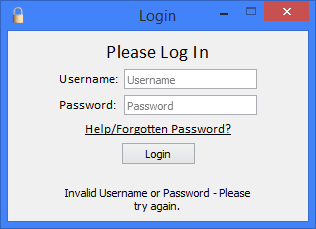
\includegraphics[width=\textwidth]{./Testing/Evidence/LoginTestFail.png}
    \caption{Test 1.1}  \label{fig:LoginTestFail}
\end{figure}

\begin{figure}[H]
    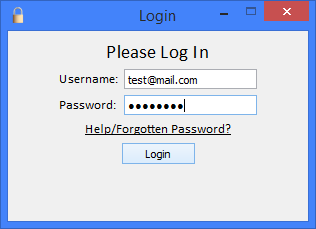
\includegraphics[width=\textwidth]{./Testing/Evidence/LoginTestSucceed.png}
    \caption{Test 1.2}  \label{fig:LoginTestSucceed}
\end{figure}

\end{landscape}

\section{Evaluation}

\subsection{Approach to Testing}

\subsection{Problems Encountered}

\subsection{Strengths of Testing}

\subsection{Weaknesses of Testing}

\subsection{Reliability of Application}

\subsection{Robustness of Application}